% Created 2016-08-17 Wed 14:38
\documentclass[tikz]{standalone}

\usepackage[utf8]{inputenc}
\usepackage[T1]{fontenc}

\usepackage{circledsteps}

\RequirePackage{xcolor}

%% HPI color definitions according to the design manual
% These do not exactly match the RGB values used in the Powerpoint slide master due to unknown reasons
\definecolor{hpiyellow}{RGB}{246,168,0}
\definecolor{hpiorange}{RGB}{221,97,8}
\definecolor{hpired}{RGB}{177,6,58}
\definecolor{hpigray}{RGB}{90,96,101}
\definecolor{hpiblue}{RGB}{0,122,158}


\renewcommand{\sfdefault}{neosans}
% Different font weights for neosans
\newcommand{\textl}[1]{{\fontseries{l}\selectfont #1}} % light
\newcommand{\textm}[1]{{\fontseries{m}\selectfont #1}} % medium, same as default weight
\newcommand{\textsb}[1]{{\fontseries{sb}\selectfont #1}} % semibold
\newcommand{\textmb}[1]{{\fontseries{mb}\selectfont #1}} % bold, same as \textbf
\newcommand{\texteb}[1]{{\fontseries{eb}\selectfont #1}} % extra bold
\newcommand{\textub}[1]{{\fontseries{ub}\selectfont #1}} % ultra bold

\tikzset{every picture/.style={/utils/exec={\sffamily}}}
\tikzset{flipflop RSflanke/.style={
  flipflop,
  flipflop def={t1=S, t2=C, c2=1, t3=R, t6=Q, t4={\ctikztextnot{Q}}}
}}


\tikzset{
  mechanicalSwitch/.pic={
    \coordinate (-inUp) at (135:2); 
    \coordinate (-inDown) at (235:2);
    \coordinate (-out) at (2,0);
    \coordinate (-center) at (0,0);
    
    \draw (0,0) circle [radius = 2cm];
    \draw [fill=gray!20] (0,0) circle [radius = 0.2cm];

    \draw (0, 0) -- (2, 0);
    \draw (135:.8) -- (135:2); 
    \draw (225:.8) -- (225:2); 

    \draw [fill=gray!20] (2, 0) circle [radius=0.05cm]; 
    \draw [fill=gray!20] (135:2) circle [radius=0.05cm]; 
    \draw [fill=gray!20] (225:2) circle [radius=0.05cm]; 

    
    \draw [thick] (0,0) -- (175:1.5); 

    \draw [dashed, <->, domain=135:225] plot ({cos(\x)}, {sin(\x)}); 
  },
  mechanicalSwitchClosed/.pic={
    \coordinate (-inUp) at (135:2); 
    \coordinate (-inDown) at (255:2);
    \coordinate (-out) at (2,0);
    \coordinate (-center) at (0,0);
    \draw (0,0) circle [radius = 2cm];
    \draw [fill=gray!20] (0,0) circle [radius = 0.2cm];

    \draw (0, 0) -- (2, 0);
    \draw (135:.8) -- (135:2); 
    \draw (225:.8) -- (225:2); 

    \draw [fill=gray!20] (2, 0) circle [radius=0.05cm]; 
    \draw [fill=gray!20] (135:2) circle [radius=0.05cm]; 
    \draw [fill=gray!20] (225:2) circle [radius=0.05cm]; 

    
    \draw [thick] (0,0) -- (135:2); 

    \draw [dashed, <->, domain=135:225] plot ({cos(\x)}, {sin(\x)}); 
  }
}


\usetikzlibrary{calc}
\usetikzlibrary{positioning}


\usepackage{../../templates/moeptikz}

\usetikzlibrary{backgrounds,fit,shapes.symbols,shapes.geometric,shapes.callouts}
\usetikzlibrary {ext.positioning-plus}

\begin{document}

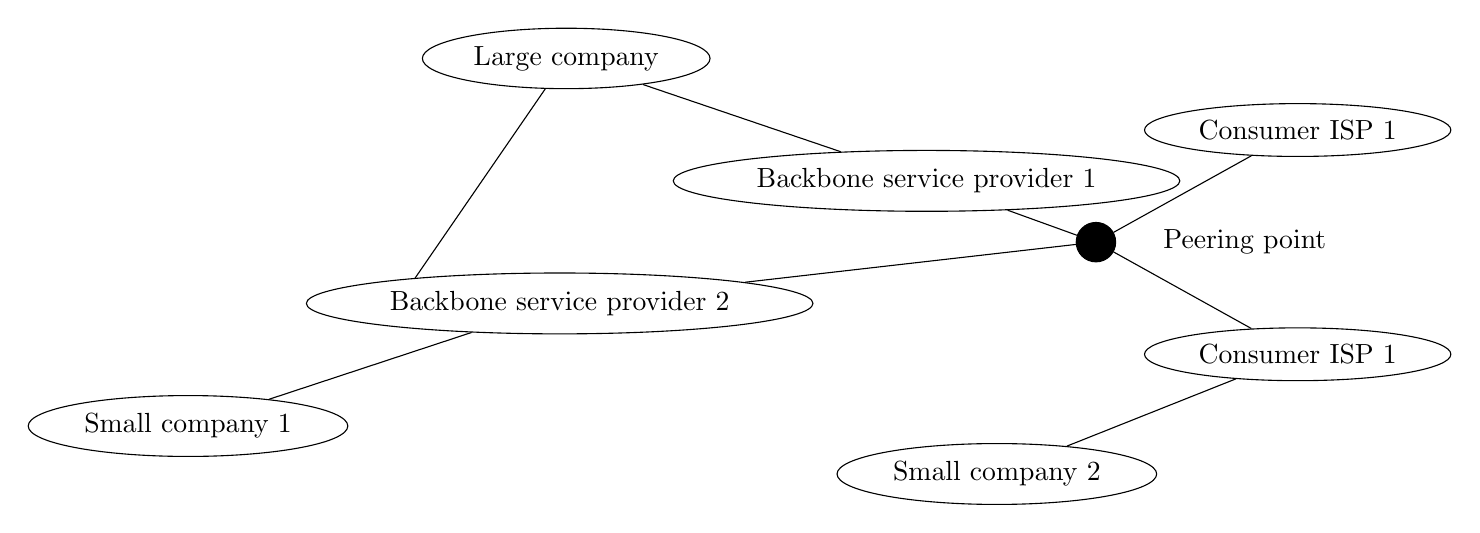
\begin{tikzpicture}[every node/.style={draw,ellipse}]
  \label{page:routing:as_structure}

  \node (bsp1) {Backbone service provider 1}; 
  \node [below left=1cm and 0.1cm of bsp1] (bsp2) {Backbone service provider 2};

  \node [above left=of bsp1] (large) {Large company}; 
  \node [below left=of bsp2] (small1) {Small company 1}; 

  \node [right=of ($(bsp1.east)!0.5!(bsp2.east)$), fill, circle, minimum width=0.5cm, label=right:Peering point] (pp) {};

  \node [above right=of pp] (isp1) {Consumer ISP 1}; 
  \node [below right=of pp] (isp2) {Consumer ISP 1}; 

  \node [below left=of isp2] (small2) {Small company 2}; 

  \draw (large) -- (bsp1) -- (pp)  -- (isp1);
  \draw (small1) -- (bsp2)  --  (pp)  -- (isp2) -- (small2);
  \draw (bsp2.170) -- (large); 
  
  
\end{tikzpicture}

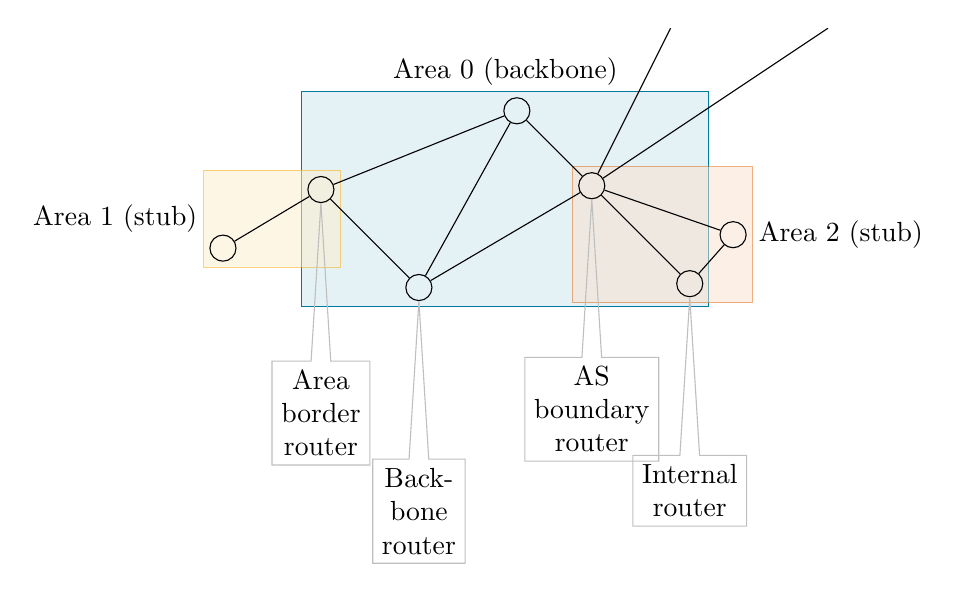
\begin{tikzpicture}
  \label{page:routing:ospf_areas}

  \begin{scope}[every node/.style={draw, circle}]
    \node (n1) {}; 
    \node [above right=0.5cm and 1cm of n1] (n2) {};
    \node [below right=of n2] (n3) {};
    \node [above right=2cm and 1cm of n3] (n4) {};
    \node [below right =1cm of n4] (n5) {};
    \node [below right=of n5] (n6) {};
    \node [right=of ($(n5)!0.5!(n6)$)] (n7) {}; 
  \end{scope}

  \draw (n1) -- (n2) edge (n3) -- (n4) edge (n3) -- (n5) edge (n3) edge (n6) -- (n7) edge (n6); 
  \draw (n5) edge ++(1,2) edge ++(3, 2); 
  
  \begin{scope}[every node/.style={rectangle}, on background layer, inner sep=2pt]
    \node [fit=(n2)(n3)(n4)(n5)(n6), label=above:Area 0 (backbone), draw=hpiblue, fill=hpiblue!10] {}; 
    \node [fit=(n1)(n2), label=left:Area 1 (stub), fill=hpiyellow!20, draw=hpiyellow, semitransparent] {}; 
    \node [fit=(n7)(n5)(n6), label=right:Area 2 (stub), draw=hpiorange, fill=hpiorange!20, semitransparent] {}; 
  \end{scope}

  \begin{scope}[every node/.style={rectangle callout, draw=gray!50, align=center, }]
    \node [callout absolute pointer={(n2.south)}, below=2cm of n2] {Area \\border\\ router};     
    \node [callout absolute pointer={(n3.south)}, below=2cm of n3] {Back-\\bone\\ router}; 
    \node [callout absolute pointer={(n5.south)}, below=2cm of n5] {AS\\boundary\\ router}; 
    \node [callout absolute pointer={(n6.south)}, below=2cm of n6] {Internal\\ router}; 
  \end{scope}
  
  
\end{tikzpicture}



% -------------------------------

% BGP: core scenario


\newcommand{\bgpcore}[0]{  \begin{scope}
    \node [router] (r1c) {R1c}; 
    \node [router, right=of r1c] (r1a) {R1a}; 
    \node [router, below=of r1c] (r1d) {R1d}; 
    \node [router, below=of r1a] (r1b) {R1b};
    \node [below=0.5cm of r1b] (bugfix) {};
    \scoped[on background layer] {\node [fill=hpiyellow!10,draw=hpiyellow, fit=(r1a)(r1b)(r1c)(r1d)(bugfix),label=below:AS 1]  {}; }

    \draw (r1c) --(r1a)  (r1d) -- (r1b); 
  \end{scope}

  \begin{scope}[xshift=6cm,yshift=-1cm]
    \node [router] (r2c) {R2c}; 
    \node [router, right=of r2c] (r2a) {R2a}; 
    \node [router, below=of r2c] (r2d) {R2d}; 
    \node [router, below=of r2a] (r2b) {R2b};
    \node [below=0.5cm of r2b] (bugfix) {};
    \scoped[on background layer] {\node [fill=hpired!10,draw=hpired, fit=(r2a)(r2b)(r2c)(r2d)(bugfix),label=below:AS 2]  {}; }
    \draw (r2c) edge (r2d) --(r2a) (r2b) -- (r2c); 
  \end{scope}

  \begin{scope}[xshift=12cm,yshift=0cm]
    \node [router] (r3c) {R3c}; 
    \node [router, right=of r3c] (r3a) {R3a}; 
    \node [router, below=of r3c] (r3d) {R3d}; 
    \node [router, below=of r3a] (r3b) {R3b};
    \node [below=0.5cm of r3b] (bugfix) {};
    \scoped[on background layer] {\node [fill=hpiorange!10,draw=hpiorange, fit=(r3a)(r3b)(r3c)(r3d)(bugfix),label=below:AS 3]  {}; }
    \draw (r3c)  --(r3a) edge (r3d) -- (r3b) -- (r3d); 
  \end{scope}

  \draw (r1a) -- (r2c) (r1b) -- (r2d) (r2a) -- (r3c) (r2b) -- (r3d); 

  \begin{scope}[every node/.style={circle, draw}]
    \node [above left=of r1c](a){A};
    \node [below left=of r1d](b){B};
    \node [right=of r3a](c){C};
    \node [right=of r3b](d){D};

    \draw (a) -- (r1c) (b) -- (r1d) (c) -- (r3a) (d) -- (r3b); 
  \end{scope}
  
}


\newcommand{\bgpstructuredprefix}[0]{  \begin{scope}[every node/.append style={align=left, anchor=west}]
    \node [above right=0.25cm of c, ] (prefixes_at_c_1) {138.13.64/24};
    \node [below right=0.25cm of c, ] (prefixes_at_c_2) {138.13.65/24};
    
    \node [above right=0.25cm of d, ] (prefixes_at_d_1) {138.13.66/24};
    \node [below right=0.25cm of d, ] (prefixes_at_d_2) {138.13.67/24};
  \end{scope}

  \draw (prefixes_at_c_1) -- (c) -- (prefixes_at_c_2); 
  \draw (prefixes_at_d_1) -- (d) -- (prefixes_at_d_2);
}

\newcommand{\movedprefix}[0]{  \begin{scope}[every node/.append style={align=left, anchor=west}]
    \node [above right=0.25cm of c, ] (prefixes_at_c_1) {138.13.64/24};
    \node [below right=0.25cm of c, ] (prefixes_at_c_2) {138.13.65/24};
    
    \node [above right=0.25cm of d, ] (prefixes_at_d_1) {138.13.66/24};
    \node [below right=0.25cm of b, ] (prefixes_at_d_2) {138.13.67/24};
  \end{scope}

  \draw (prefixes_at_c_1) -- (c) -- (prefixes_at_c_2); 
  \draw (prefixes_at_d_1) -- (d) (b) -- (prefixes_at_d_2);
}


\begin{tikzpicture}
  \label{page:routing:bgpcore}
  \bgpcore 
\end{tikzpicture}

\begin{tikzpicture}
  \label{page:routing:bgp:simpleprefix}
  \bgpcore

  \bgpstructuredprefix
  
  \begin{scope}[every node/.style={rectangle callout, draw=gray!50, align=center, }]
    \node [callout absolute pointer={(r3c.west)}, above=2cm of r3c.west] {Announce:\\138.13.64/22};     
    \node [callout absolute pointer={(r3d.west)}, below=2cm of r3d.west] {Announce:\\138.13.64/22};     
  \end{scope}
  
\end{tikzpicture} 

\begin{tikzpicture}
  \label{page:routing:bgp:movedprefix}
  \bgpcore

  \movedprefix
  
  \begin{scope}[every node/.style={rectangle callout, draw=gray!50, align=center, }]
    \node [callout absolute pointer={(r3c.west)}, above=2cm of r3c.west] {Announce:\\138.13.64/22};     
    \node [callout absolute pointer={(r3d.west)}, below=2cm of r3d.west] {Announce:\\138.13.64/22};     
    \node [callout absolute pointer={(r1a.east)}, above=2cm of r1a.east] {Announce:\\138.13.67/24};     

  \end{scope}
  
\end{tikzpicture} 


\begin{tikzpicture}
  \label{page:routing:bgp_path}

  \bgpcore

  \bgpstructuredprefix

  % exterior BGP: 
  \begin{scope}[every node/.style={rectangle callout, draw=gray!50, align=left, fill=hpiblue!10 }]
    \node [callout absolute pointer={(r3c.west)}, above=2cm of r3c.west]
    {Announce:\\
      Prefix:  138.13.64/22 \\
      AS-Path: AS3 \\
      Next hop: R3c (west interface)};

    \node [callout absolute pointer={(r3d.west)}, below=2cm of r3d.west]
    {Announce:\\
      Prefix:  138.13.64/22 \\
      AS-Path: AS3 \\
      Next hop: R3d (west interface)};


    \node [callout absolute pointer={(r2c.west)}, above=2cm of r2c.west]
    {Announce:\\
      Prefix:  138.13.64/22 \\
      AS-Path: AS2, AS3 \\
      Next hop: R2c (west interface)};

    \node [callout absolute pointer={(r2d.west)}, below=2cm of r2d.west]
    {Announce:\\
      Prefix:  138.13.64/22 \\
      AS-Path: AS2, AS3 \\
      Next hop: R2d (west interface)};

  \end{scope}
  
  % interior BGP: 
\begin{scope}[every node/.style={rectangle callout, draw=gray!50, align=left, fill=hpiblue!50 }]

    \node [callout absolute pointer={(r1c.west)}, above=2cm of r1c.west]
    {Announce:\\
      Prefix:  138.13.64/22 \\
      AS-Path: AS2, AS3 \\
      Next hop: \textbf{R1a (east interface)}};

    \node [callout absolute pointer={(r1d.west)}, below=2cm of r1d.west]
    {Announce:\\
      Prefix:  138.13.64/22 \\
      AS-Path: AS2, AS3 \\
      Next hop: \textbf{R1b (east interface)}};

  \end{scope}
  
\end{tikzpicture}



\end{document}